% 1988 年上海卷第五题：正四面体 A-BCD，E/F 为中点
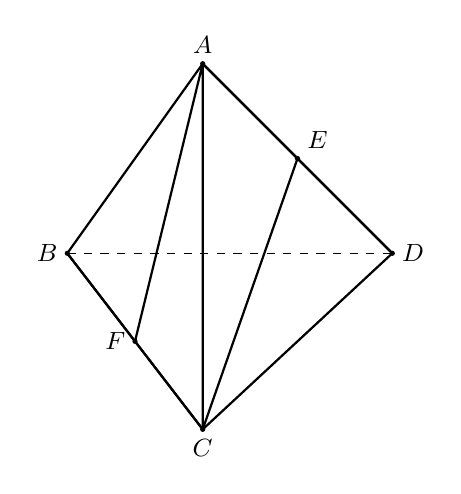
\begin{tikzpicture}[scale=0.86,>=stealth,font=\small]
  \coordinate (A) at (0,3.8);
  \coordinate (B) at (-2.0,1.0);
  \coordinate (C) at (0,-1.6);
  \coordinate (D) at (2.8,1.0);
  \coordinate (E) at (1.4,2.4);
  \coordinate (F) at (-1.0,-0.3);
  \draw[thick] (A)--(B)--(C)--(D)--cycle;
  \draw[thick] (A)--(C) (A)--(F) (C)--(E);
  \draw[dashed] (B)--(D);
  \draw[thick] (B)--(F)--(C);
  \draw[thick] (A)--(E)--(D);
  \fill (A) circle (1.1pt) node[above] {$A$};
  \fill (B) circle (1.1pt) node[left] {$B$};
  \fill (C) circle (1.1pt) node[below] {$C$};
  \fill (D) circle (1.1pt) node[right] {$D$};
  \fill (E) circle (1.1pt) node[above right] {$E$};
  \fill (F) circle (1.1pt) node[left] {$F$};
\end{tikzpicture}
